% Figura 1 del capitolo 3: la pipeline di PGE.
% Compilare con XeLaTeX (font Liberation, come il documento):
%   xelatex -output-directory=/tmp/pipeline pipeline.tex && cp /tmp/pipeline/pipeline.pdf ../../docs/images/
\documentclass[10pt,border=3pt]{standalone}
\usepackage{fontspec}
\setmainfont{Liberation Sans}
\setsansfont{Liberation Sans}
\setmonofont{Liberation Mono}[Scale=MatchLowercase]
\renewcommand{\familydefault}{\sfdefault}
\usepackage{xcolor}
\usepackage{tikz}
\usetikzlibrary{arrows.meta,decorations.pathreplacing}

\hyphenpenalty=10000 \exhyphenpenalty=10000
\definecolor{ink}{gray}{0.08}
\definecolor{richiesta}{RGB}{170,70,0}

\tikzset{
  every node/.style={font=\small, text=ink},
  box/.style={rectangle, rounded corners=2pt, draw=ink, line width=0.5pt,
              fill=white, align=center, inner sep=3pt, minimum height=0.95cm},
  dato/.style={box, line width=1.1pt, fill=black!14},
  nota/.style={anchor=west, align=left, text width=8.6cm, inner sep=0pt},
  flusso/.style={-{Stealth[length=4.5pt]}, line width=0.6pt, draw=ink},
  lettura/.style={-{Stealth[length=4.5pt]}, line width=0.6pt, draw=ink, densely dotted},
  richiesta/.style={-{Stealth[length=4.5pt]}, line width=0.8pt, draw=richiesta, dashed},
  fase/.style={decorate, decoration={brace, amplitude=4pt}, line width=0.5pt, draw=black!60},
  fasetesto/.style={rotate=90, anchor=south, font=\footnotesize\bfseries}
}

\begin{document}
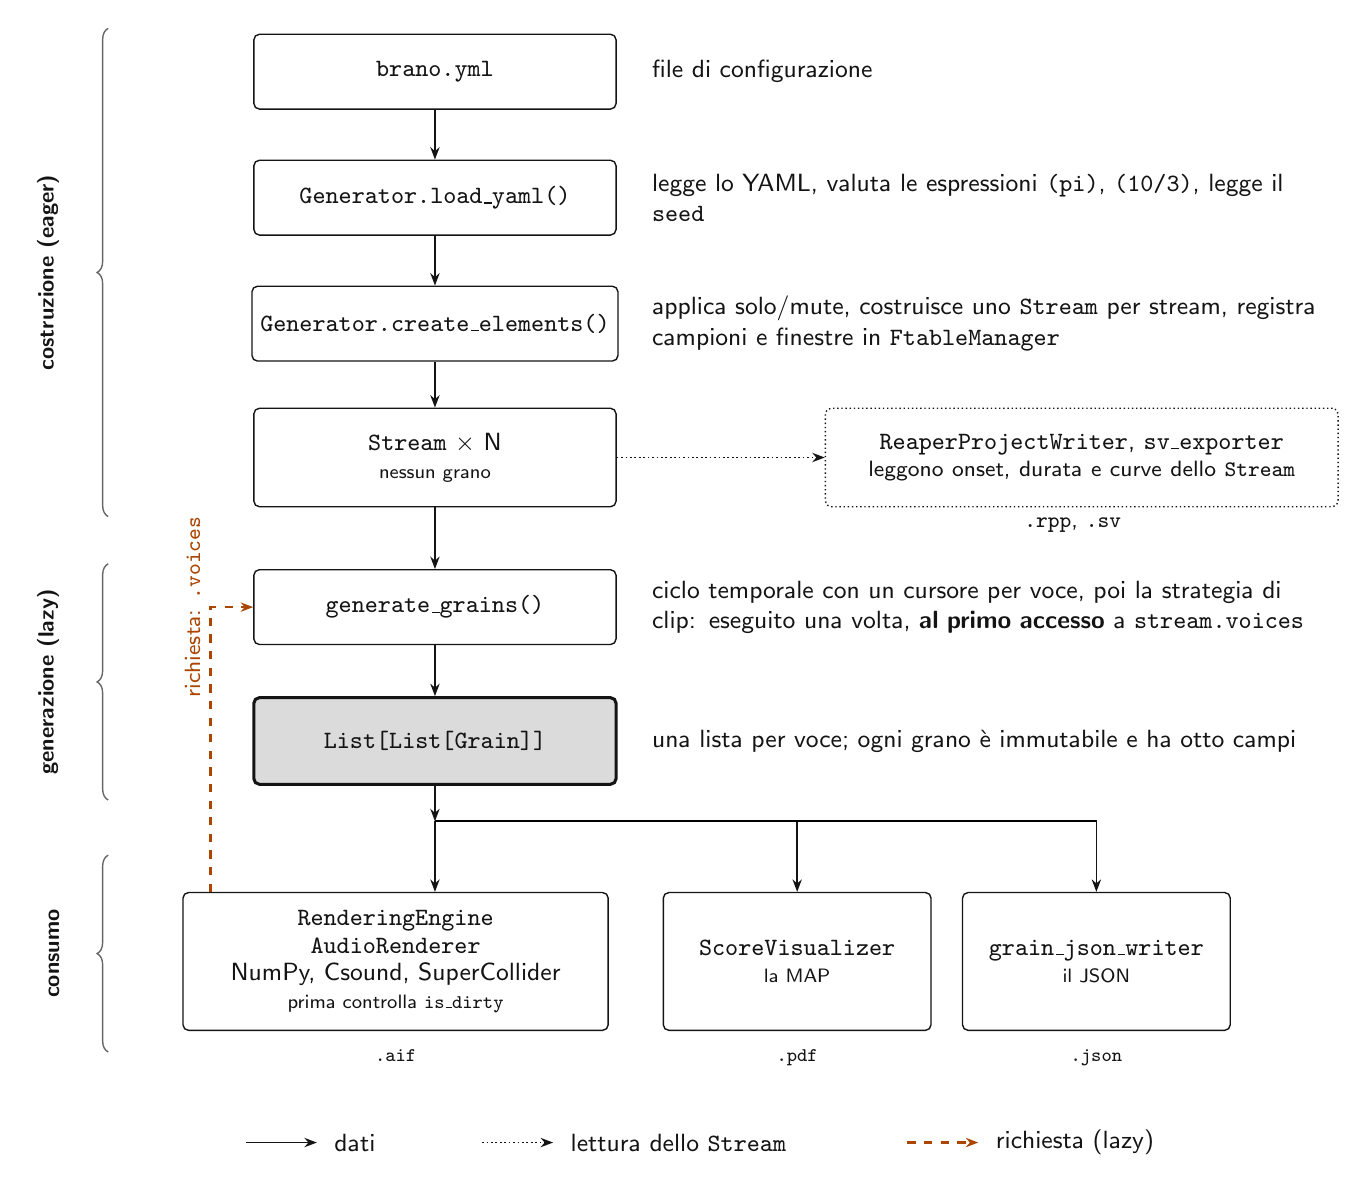
\begin{tikzpicture}[x=1cm,y=1cm]

% --- colonna principale -----------------------------------------------------
\node[box, minimum width=4.6cm] (yaml)   at (3.6, 0)    {\texttt{brano.yml}};
\node[box, minimum width=4.6cm] (load)   at (3.6,-1.6)  {\texttt{Generator.load\_yaml()}};
\node[box, minimum width=4.6cm] (create) at (3.6,-3.2)  {\texttt{Generator.create\_elements()}};
\node[box, minimum width=4.6cm, minimum height=1.25cm] (stream) at (3.6,-4.9)
      {\texttt{Stream} $\times$ N\\[-1pt]{\scriptsize nessun grano}};
\node[box, minimum width=4.6cm] (gen)    at (3.6,-6.8)  {\texttt{generate\_grains()}};
\node[dato, minimum width=4.6cm, minimum height=1.1cm] (lista) at (3.6,-8.5)
      {\texttt{List[List[Grain]]}};

% --- note a destra ----------------------------------------------------------
\node[nota] at (6.35, 0)    {file di configurazione};
\node[nota] at (6.35,-1.6)  {legge lo YAML, valuta le espressioni \texttt{(pi)}, \texttt{(10/3)}, legge il \texttt{seed}};
\node[nota] at (6.35,-3.2)  {applica solo/mute, costruisce uno \texttt{Stream} per stream, registra campioni e finestre in \texttt{FtableManager}};
\node[nota] at (6.35,-6.8)  {ciclo temporale con un cursore per voce, poi la strategia di clip: eseguito una volta, \textbf{al primo accesso} a \texttt{stream.voices}};
\node[nota] at (6.35,-8.5)  {una lista per voce; ogni grano è immutabile e ha otto campi};

% --- consumatori di Stream --------------------------------------------------
\node[box, anchor=west, text width=6.3cm, minimum height=1.25cm, densely dotted] (rs) at (8.55,-4.9)
      {\texttt{ReaperProjectWriter}, \texttt{sv\_exporter}\\[-1pt]{\footnotesize leggono onset, durata e curve dello \texttt{Stream}}};

% --- consumatori della lista ------------------------------------------------
\node[box, minimum width=5.4cm, minimum height=1.75cm] (c1) at (3.1,-11.3)
      {\texttt{RenderingEngine}\\[-1pt]\texttt{AudioRenderer}\\[-1pt]NumPy, Csound, SuperCollider\\[-1pt]{\scriptsize prima controlla \texttt{is\_dirty}}};
\node[box, minimum width=3.4cm, minimum height=1.75cm] (c2) at (8.2,-11.3)
      {\texttt{ScoreVisualizer}\\[-1pt]{\scriptsize la MAP}};
\node[box, minimum width=3.4cm, minimum height=1.75cm] (c3) at (12.0,-11.3)
      {\texttt{grain\_json\_writer}\\[-1pt]{\scriptsize il JSON}};

\node[anchor=north, font=\scriptsize] at (3.1,-12.3)  {\texttt{.aif}};
\node[anchor=north, font=\scriptsize] at (8.2,-12.3)  {\texttt{.pdf}};
\node[anchor=north, font=\scriptsize] at (12.0,-12.3) {\texttt{.json}};
\node[anchor=north, font=\footnotesize] at (11.7,-5.55)  {\texttt{.rpp}, \texttt{.sv}};

% --- frecce dei dati --------------------------------------------------------
\draw[flusso] (yaml)   -- (load);
\draw[flusso] (load)   -- (create);
\draw[flusso] (create) -- (stream);
\draw[flusso] (stream) -- (gen);
\draw[flusso] (gen)    -- (lista);
\draw[lettura] (stream.east) -- (rs.west);

\draw[flusso] (lista.south) -- ++(0,-0.45) coordinate (bus);
\draw[flusso] (bus) -| (c1.north -| lista);
\draw[flusso] (bus) -| (c2.north);
\draw[flusso] (bus) -| (c3.north);
\draw[line width=0.6pt] (bus) -- (c3.north |- bus);

% --- la richiesta (pull) ----------------------------------------------------
\draw[richiesta] ([xshift=-2.35cm]c1.north) |- (gen.west)
      node[pos=0.5, rotate=90, anchor=south, text=richiesta, font=\footnotesize]
      {richiesta: \texttt{.voices}};

% --- fasi -------------------------------------------------------------------
\draw[fase] (-0.55,-5.65) -- (-0.55, 0.55);
\node[fasetesto] at (-1.05,-2.55) {costruzione (eager)};
\draw[fase] (-0.55,-9.25) -- (-0.55,-6.25);
\node[fasetesto] at (-1.05,-7.75) {generazione (lazy)};
\draw[fase] (-0.55,-12.45) -- (-0.55,-9.95);
\node[fasetesto] at (-1.05,-11.2) {consumo};

% --- legenda ----------------------------------------------------------------
\begin{scope}[shift={(1.2,-13.6)}, font=\scriptsize]
  \draw[flusso] (0,0) -- (0.9,0);                  \node[anchor=west] at (1.0,0) {dati};
  \draw[lettura] (3.0,0) -- (3.9,0);               \node[anchor=west] at (4.0,0) {lettura dello \texttt{Stream}};
  \draw[richiesta] (8.4,0) -- (9.3,0);             \node[anchor=west] at (9.4,0) {richiesta (lazy)};
\end{scope}

\end{tikzpicture}
\end{document}
